\documentclass[12pt]{article}
\usepackage[utf8]{inputenc}
\usepackage[T1]{fontenc}
\usepackage{amsmath,amssymb,amsthm}
\usepackage{graphicx}
\usepackage[margin=1in]{geometry}
\usepackage{hyperref}
\usepackage{booktabs}
\usepackage{natbib}
\usepackage[nopatch=footnote]{microtype}

\newtheorem{theorem}{Theorem}
\newtheorem{lemma}[theorem]{Lemma}
\newtheorem{corollary}[theorem]{Corollary}
\newtheorem{proposition}[theorem]{Proposition}
\theoremstyle{definition}
\newtheorem{definition}[theorem]{Definition}
\theoremstyle{remark}
\newtheorem{remark}[theorem]{Remark}

\DeclareMathOperator{\Tr}{Tr}
\DeclareMathOperator{\tr}{tr}
\DeclareMathOperator{\Ric}{Ric}
\DeclareMathOperator{\Vol}{Vol}
\DeclareMathOperator{\Spin}{Spin}
\DeclareMathOperator{\SU}{SU}
\DeclareMathOperator{\Sp}{Sp}
\DeclareMathOperator{\sgn}{sgn}
\DeclareMathOperator{\Spec}{Spec}
\DeclareMathOperator{\Cliff}{Cl}
\DeclareMathOperator{\ad}{ad}
\DeclareMathOperator{\End}{End}
\DeclareMathOperator{\Cas}{Cas}

\title{Monotonicity of the Spectral Action Under Volume-Preserving Deformations of SU(3)}
\author{MemeTheory\thanks{AI assistance in research and manuscript
  preparation (Anthropic Claude: Opus 4.6--4.8, Fable 5).}}
\date{\today}

\begin{document}

\maketitle

\begin{abstract}
We study the spectral action functional $\Tr f(D^2/\Lambda^2)$ on the
compact Lie group $\SU(3)$ equipped with a one-parameter family of
volume-preserving left-invariant metrics --- the Jensen deformation ---
which interpolates between the bi-invariant round metric ($\tau=0$) and
a squashed metric that breaks the symmetry from $\SU(3)\times\SU(3)$
to $\SU(3)\times U(2)$.  We establish the following results.
First, the geometric Seeley--DeWitt coefficient $a_2(\tau)$,
proportional to the scalar curvature integral, is analytically proven
to be monotonically increasing along the Jensen curve
(Proposition~\ref{prop:R-monotone}).
Second, the multiplicity-weighted mean eigenvalue squared
$\langle\lambda^2\rangle(\tau)$ increases monotonically from $2.495$
at $\tau=0$ to $3.471$ at $\tau=0.5$, and each of the $10$
Peter--Weyl sectors (representations with $p+q\leq 3$) is
individually monotone in the same direction; this monotonicity is
established not only numerically but as a closed-form, truncation-uniform
sign identity (Theorem~\ref{thm:structural}).
Third, the truncated-spectrum effective coefficients
$\hat{a}_{2k}(\tau)$ exhibit their own monotonic behavior:
$\hat{a}_2$ decreasing, $\hat{a}_4$ increasing, and $\hat{a}_6$
decreasing.
Fourth, for all \emph{completely monotone} cutoff functions $f$
(satisfying $(-1)^n f^{(n)} \geq 0$, a class including Gaussian,
exponential, and heat kernel cutoffs), $S_f(\tau)$ is strictly
monotone in $\tau$ with no interior critical point --- decreasing for
$f$ decreasing, increasing for $f$ increasing --- and this
absence of an interior extremum is robust to the one-loop correction.
Computational verification confirms strict monotonicity for $10$
representative cutoff functions spanning Gaussian, exponential, and
power-law families.
Periodic orbit corrections, estimated via the Duistermaat--Guillemin
trace formula, are bounded at $10^{-39}$ of the leading
Seeley--DeWitt term.  As a comparison, the analogous spectral action
on the dimension-matched space $\SU(2)\times\SU(2)$ with Berger
deformation has $d^2S/d\tau^2 = -3.42$ (concave down, no folds),
while $\SU(3)$ has $d^2S/d\tau^2 = +20.42$ (concave up, eigenvalue
fold), demonstrating that the monotonicity is controlled by
representation-theoretic properties specific to $\SU(3)$.  These
results provide partial progress toward the open problem, noted by
Connes in 2019, of understanding the spectral action under general
metric deformations, for one specific deformation family on one
manifold.  Because the action is a strictly monotone function of the
modulus with no stationary point, the deformation parameter is not
stabilized by the spectral action: it is a flowing modulus, and the
monotone gradient is precisely what drives that flow.
\end{abstract}

%% ====================================================================
\section{Introduction}
%% ====================================================================

The spectral action principle, introduced by Chamseddine and Connes
\cite{Chamseddine1997}, asserts that the physical
action for a noncommutative geometry described by a spectral triple
$(\mathcal{A}, \mathcal{H}, D)$ takes the form
\begin{equation}\label{eq:spectral-action-def}
  S_f(\Lambda) \;=\; \Tr\, f\!\left(\frac{D^2}{\Lambda^2}\right),
\end{equation}
where $f$ is a suitable cutoff function and $\Lambda$ is an energy
scale.  When the spectral triple encodes a Riemannian spin manifold
$M$, the asymptotic expansion of \eqref{eq:spectral-action-def} in
powers of $\Lambda^{-1}$ recovers the Einstein--Hilbert action, the
cosmological constant, and higher-curvature corrections, with
coefficients given by the Seeley--DeWitt invariants $a_{2k}$ of
$D^2$ \cite{Gilkey1995, Vassilevich2003}.  When
$M$ is replaced by a product $M^4 \times K$ with a compact internal
space $K$, dimensional reduction produces the bosonic sector of the
Standard Model coupled to gravity
\cite{ChamseddineConnesMarcolli2007,
  vanSuijlekom2015}.

A fundamental open problem in this program is how the spectral action
depends on the choice of metric on $K$.  Connes observed in his 2019
review \cite{Connes2019} that ``the problem of encoding
a general change of metric remains open.''  The spectral action is
defined for a given spectral triple, and hence for a given
metric on $K$; but if the geometry of $K$ is to be
determined dynamically --- as a modulus stabilized at a minimum of
$S_f$ --- then one needs to understand how $S_f$ varies as the metric
changes.  Inner fluctuations of the Dirac operator (the
noncommutative analogue of gauge transformations) are well understood
\cite{ChamseddineConnesvanSuijlekom2013}, but metric deformations that
alter the Riemannian geometry of $K$ lie outside the inner
fluctuation formalism.  As we show below, for the deformation family
studied here \emph{no} such minimum exists: the spectral action is a
strictly monotone function of the modulus with no stationary point.
Section~\ref{sec:consequences} discusses why this is structurally
expected, and what it implies --- that the modulus is not stabilized
by the spectral action but flows under its monotone gradient.

This paper addresses the problem for a specific but important case:
$K = \SU(3)$, the compact simple Lie group of dimension $8$ and
rank $2$, equipped with the Jensen one-parameter family of
volume-preserving left-invariant metrics.  The Jensen deformation is
the unique (up to scale) one-parameter curve in the moduli space of
$U(2)$-invariant left-invariant metrics on $\SU(3)$ that preserves
the Riemannian volume
\cite{Jensen1973, Baptista2024}.  At
$\tau = 0$ the metric is bi-invariant (the round metric), and for
$\tau > 0$ the isometry group breaks from
$\SU(3) \times \SU(3)$ to $\SU(3) \times U(2)$.  The space
$\SU(3)$ plays a distinguished role in Kaluza--Klein
compactifications: it is the internal manifold in several models of
particle physics from extra dimensions
\cite{Baptista2024, Witten1981}, and its spectrum
produces the Standard Model quantum numbers when combined with the
appropriate finite spectral triple
\cite{ChamseddineConnesMarcolli2007}.

The Dirac operator $D_K(\tau)$ on $(\SU(3), g_\tau)$ can be
decomposed via the Peter--Weyl theorem into finite matrix problems,
one for each irreducible representation of $\SU(3)$.  This
block-diagonalization follows from Schur's lemma applied to the
equivariant structure of the Dirac operator on a compact Lie group ---
it is a standard result in spectral geometry of homogeneous spaces
\cite{Fegan1987, Slebarski1985,
  Bar1992}.  The full spectrum is the union of eigenvalues
across all representation sectors, each appearing with Peter--Weyl
multiplicity $\dim(\pi)^2$.

\medskip

\noindent\textbf{Contributions.}  This paper establishes the following
results:

\begin{enumerate}
\item \textbf{Seeley--DeWitt monotonicity (Theorem~\ref{thm:SD-mono}).}
  The coefficients $a_0(\tau)$, $a_2(\tau)$, $a_4(\tau)$, $a_6(\tau)$,
  extracted from the small-$t$ asymptotic expansion of the heat trace
  $\Tr e^{-tD_K^2}$, are individually monotone functions of $\tau$ on
  $[0,\, 0.5]$.  The geometric coefficient $a_2 \propto \mathcal{R}$
  is increasing, and $a_4 \propto 5\mathcal{R}^2 - 2|\Ric|^2 +
  2|\mathrm{Riem}|^2$ is non-decreasing, with derivative vanishing
  only at the bi-invariant point $\tau=0$ and strictly positive for
  $\tau>0$.

\item \textbf{Structural monotonicity (Theorem~\ref{thm:structural}).}
  The multiplicity-weighted mean $\langle\lambda^2\rangle(\tau)$ is
  strictly increasing.  Each of the $10$ Peter--Weyl sectors with
  $p+q \leq 3$ (comprising $155{,}984$ weighted modes) is
  individually monotone in the same direction; we give a closed-form,
  truncation-uniform sign identity establishing
  $d\langle\lambda^2\rangle/d\tau > 0$ for all $\tau>0$ at every
  truncation level.  For all completely monotone cutoff functions $f$
  and any $\Lambda > 0$, the spectral action $S_f(\tau)$ is strictly
  monotone with no interior critical point.  Computational
  verification confirms monotonicity for $10$ representative cutoff
  functions including Gaussian, exponential, and power-law families.
  No local extremum exists on $[0,\,0.5]$ for any tested cutoff.

\item \textbf{Periodic orbit bound (Proposition~\ref{prop:periodic}).}
  Duistermaat--Guillemin oscillatory corrections to the spectral
  action are bounded at $10^{-39}$ relative to the leading
  Seeley--DeWitt term, confirming that the perturbative heat kernel
  expansion is exact to at least $39$ decimal places on the Jensen
  curve.

\item \textbf{SU(3) specificity
  (Proposition~\ref{prop:specificity}).}  On the
  dimension-matched alternative $\SU(2)\times\SU(2)$ with Berger
  deformation, the spectral action curvature is $d^2S/d\tau^2 =
  -3.42 < 0$ (no folds, concave down), while on $\SU(3)$ it is
  $+20.42 > 0$ (eigenvalue fold, concave up).  The sign difference
  traces to the existence of complex representations in $\SU(3)$
  versus only real and pseudoreal representations in $\SU(2)$.
\end{enumerate}

The remainder of the paper is organized as follows.
Section~\ref{sec:prelim} recalls the necessary background on spectral
triples, the spectral action, and Seeley--DeWitt coefficients.
Section~\ref{sec:jensen} constructs the Jensen deformation and the
Dirac operator on $\SU(3)$.  Section~\ref{sec:SD-mono} proves the
monotonicity of the Seeley--DeWitt coefficients (Theorem~A).
Section~\ref{sec:structural} proves the structural monotonicity
theorem (Theorem~B) and bounds the periodic orbit corrections.
Section~\ref{sec:consequences} discusses consequences for moduli
dynamics and places the results in the context of Connes' open
problem.  The appendix details the computational methodology.


%% ====================================================================
\section{Preliminaries}\label{sec:prelim}
%% ====================================================================

\subsection{Spectral triples and the spectral action}

A \emph{spectral triple} $(\mathcal{A}, \mathcal{H}, D)$ consists of a
$*$-algebra $\mathcal{A}$ represented faithfully on a Hilbert space
$\mathcal{H}$, together with a self-adjoint operator $D$ on
$\mathcal{H}$ (the \emph{Dirac operator}) such that
$[D, a]$ is bounded for all $a \in \mathcal{A}$ and $(D + i)^{-1}$ is
compact \cite{Connes1994}.  In the commutative case,
$\mathcal{A} = C^\infty(M)$ for a closed Riemannian spin manifold $M$,
$\mathcal{H} = L^2(M, S)$ is the Hilbert space of $L^2$ spinor
fields, and $D$ is the Atiyah--Singer Dirac operator
\cite{LawsonMichelsohn1989}.

Given a positive even function $f$ with sufficient decay at infinity,
the \emph{spectral action} is the trace
\begin{equation}\label{eq:spectral-action}
  S_f(\Lambda) \;=\; \Tr\, f\!\left(\frac{D^2}{\Lambda^2}\right)
  \;=\; \sum_n f\!\left(\frac{\lambda_n^2}{\Lambda^2}\right),
\end{equation}
where $\{\lambda_n\}$ are the eigenvalues of $D$ (counted with
multiplicity) and $\Lambda > 0$ is an energy cutoff.  The spectral
action is a pure functional of the spectrum $\{\lambda_n\}$: the
geometry of $M$ enters only through these eigenvalues.

\subsection{Conventions for the coefficients}
\label{subsec:conventions}

Two distinct families of $\tau$-dependent numbers appear below, and we
fix names for them once to prevent conflation.  The
\emph{geometric Seeley--DeWitt coefficients} $a_{2k}(\tau)$ are the
heat-invariants of $D_K^2$ defined by the small-$t$ expansion
\eqref{eq:heat-trace-expansion}; they are curvature polynomials
evaluated through the Gilkey formulas \cite{Gilkey1995} (equivalently,
the zeta-regularized coefficients), and they are exact functions of
$\tau$.  The \emph{effective coefficients} $\hat{a}_{2k}(\tau)$ are
obtained by polynomial fitting of the \emph{truncated} heat trace over
a finite set of Peter--Weyl sectors; they approximate the geometric
$a_{2k}$ but differ from them, in particular in sign (see
Remark~\ref{rem:effective-coefficients} and
Section~\ref{sec:SD-mono}).  Whenever a numerical value is quoted, we
state explicitly which family it belongs to.


\subsection{Seeley--DeWitt coefficients}

The heat trace of $D^2$ on a closed $d$-dimensional Riemannian
manifold has the small-$t$ asymptotic expansion
\cite{Gilkey1995, Vassilevich2003}
\begin{equation}\label{eq:heat-trace-expansion}
  \Tr\, e^{-tD^2} \;\sim\; (4\pi t)^{-d/2}
  \sum_{k=0}^{\infty} a_{2k}\, t^k,
  \qquad t \to 0^+,
\end{equation}
where the \emph{Seeley--DeWitt coefficients} $a_{2k}$ are spectral
invariants of $D^2$.  They encode local geometric information: $a_0$
is proportional to the volume, $a_2$ involves the scalar curvature,
and higher coefficients involve progressively higher curvature
invariants.

For the (squared) Dirac operator $D^2 = \nabla^*\nabla + \mathcal{R}/4$
on a spin manifold of dimension $d$ (where $\mathcal{R}$ denotes the
scalar curvature and $\nabla$ is the spin connection), the leading
coefficients are
\cite{Gilkey1995, BerlineGetzlerVergne2004}:
\begin{align}
  a_0 &= \frac{2^{\lfloor d/2\rfloor}}{(4\pi)^{d/2}} \Vol(M),
    \label{eq:a0} \\[4pt]
  a_2 &= \frac{2^{\lfloor d/2\rfloor}}{(4\pi)^{d/2}}
    \int_M \frac{\mathcal{R}}{12}\, d\mathrm{vol}_g,
    \label{eq:a2}\footnotemark
    \displaybreak[0]\\[4pt]
  a_4 &= \frac{2^{\lfloor d/2\rfloor}}{(4\pi)^{d/2}} \,
    \frac{1}{360}\int_M
    \Bigl(-12\,\Delta\mathcal{R} + 5\,\mathcal{R}^2
    - 2\,|\Ric|^2 + 2\,|\mathrm{Riem}|^2\Bigr)\, d\mathrm{vol}_g.
    \label{eq:a4}
\end{align}
\footnotetext{The coefficient $\mathcal{R}/12$ in $a_2$ follows the
convention of Gilkey \cite{Gilkey1995} (Theorem~1.7.4) for the
operator $D^2 = \nabla^*\nabla + \mathcal{R}/4$, where
$\mathcal{R}/4$ is the Lichnerowicz curvature endomorphism.
Vassilevich \cite{Vassilevich2003} writes
$a_2 \propto \int \tr(\tfrac{1}{6}\mathcal{R}\,\mathrm{id} - E)$
with $E = -\mathcal{R}/4$ for the Dirac Laplacian, giving
$\mathcal{R}/6 + \mathcal{R}/4 = 5\mathcal{R}/12$ per spinor
component, which reduces to $\mathcal{R}/12$ after accounting for the
trace over the spinor fiber (since $\tr_S(\mathrm{id}) = 2^{[d/2]}$
is already factored into the prefactor in our convention).  The
\emph{monotonicity} $da_2/d\tau > 0$ is independent of the overall
normalization since $d\mathcal{R}/d\tau > 0$
(Proposition~\ref{prop:R-monotone}).}
The prefactor $2^{\lfloor d/2\rfloor}$ is the spinor rank (dimension
of the spinor bundle fiber).  For $d=8$ (the dimension of $\SU(3)$),
the spinor rank is $2^4 = 16$.

The spectral action is related to the Seeley--DeWitt coefficients via
Mellin transform.  If $f$ is a Laplace-type cutoff, then
\begin{equation}\label{eq:SA-SD-relation}
  S_f(\Lambda) \;\sim\; \sum_{k=0}^N f_{d-2k}\, \Lambda^{d-2k}\, a_{2k}
  + O(\Lambda^{d-2N-2}),
  \qquad \Lambda \to \infty,
\end{equation}
where $f_n = \int_0^\infty f(u)\, u^{n/2-1}\, du$ are the \emph{moments}
of $f$.  For physically motivated cutoff functions (Gaussian,
smooth compact support, Connes entropy), all moments $f_n$ with $n > 0$
are positive, and $f$ is monotonically decreasing on $[0,\infty)$.


\subsection{Weyl's law and the Lichnerowicz estimate}

On a closed $d$-dimensional Riemannian manifold, the eigenvalues of
$D^2$ satisfy Weyl's asymptotic law
\cite{Ivrii2019}:
\begin{equation}\label{eq:weyl-law}
  N(\Lambda) \;:=\; \#\{n : \lambda_n^2 \leq \Lambda^2\}
  \;\sim\; C_d\, \Vol(M)\, \Lambda^d, \qquad \Lambda\to\infty,
\end{equation}
where $C_d$ depends only on $d$ and the spinor rank.  Since the Jensen
deformation is volume-preserving (Section~\ref{sec:jensen}), the
leading Weyl term is $\tau$-independent: the asymptotic counting of
eigenvalues does not change along the curve.  Only the individual
eigenvalue positions move.

If the scalar curvature satisfies $\mathcal{R} \geq \mathcal{R}_{\min} > 0$,
the Lichnerowicz estimate \cite{Lichnerowicz1958} gives
\begin{equation}\label{eq:lichnerowicz}
  \lambda_1^2 \;\geq\; \frac{\mathcal{R}_{\min}}{4}.
\end{equation}
For $\SU(3)$ with the Jensen metric at the fold $\tau = 0.190$,
$\mathcal{R} = 2.018$, and the lowest eigenvalue squared is
$\lambda_1^2 = 0.672$, giving $\lambda_1^2/(\mathcal{R}/4) = 1.33$,
comfortably satisfying the bound.

\subsection{Spectral rigidity context}
\label{subsec:rigidity}

It is worth situating the Jensen curve against known rigidity results.
Gordon and Sutton \cite{GordonSutton2010} proved that on a compact
simple Lie group the bi-invariant (more generally, naturally reductive)
metric is \emph{spectrally isolated}: it admits no nearby isospectral
left-invariant deformation.  The Jensen curve is precisely such a
deformation, and our computations confirm that it changes the spectrum
(indeed monotonically): the bi-invariant metric at $\tau=0$ is the
spectral-isolation point from which the deformation departs.  The
present work may thus be read as a quantitative refinement, for one
explicit curve on $\SU(3)$, of the qualitative statement that the
naturally reductive metric is spectrally rigid.


%% ====================================================================
\section{The Jensen Deformation of SU(3)}\label{sec:jensen}
%% ====================================================================

\subsection{Reductive decomposition and left-invariant metrics}

The Lie algebra $\mathfrak{su}(3)$ admits the reductive decomposition
\cite{Jensen1973, Baptista2024}
\begin{equation}\label{eq:reductive}
  \mathfrak{su}(3) \;=\; \mathfrak{u}(1) \oplus \mathfrak{su}(2)
  \oplus \mathbb{C}^2,
\end{equation}
where $\mathfrak{u}(2) = \mathfrak{u}(1) \oplus \mathfrak{su}(2)$ is a
maximal subalgebra and $\mathbb{C}^2$ is the complementary
$\ad(\mathfrak{u}(2))$-module.  The dimensions are
$1 + 3 + 4 = 8 = \dim\SU(3)$.  In terms of the Gell-Mann basis
$\{\lambda_1,\ldots,\lambda_8\}$, the generators $e_a = -\tfrac{i}{2}\lambda_a$
decompose as:
\begin{align}
  \mathfrak{su}(2) &:\quad e_1,\, e_2,\, e_3
    \quad\text{(indices 0, 1, 2)},\nonumber\\
  \mathbb{C}^2 &:\quad e_4,\, e_5,\, e_6,\, e_7
    \quad\text{(indices 3, 4, 5, 6)},\label{eq:decomp-indices}\\
  \mathfrak{u}(1) &:\quad e_8
    \quad\text{(index 7)}.\nonumber
\end{align}
The normalization is $\tr(e_a e_b) = -\tfrac{1}{2}\delta_{ab}$, and
the Killing form is $B_{ab} = -3\delta_{ab}$.

A $U(2)$-invariant left-invariant metric on $\SU(3)$ is specified by
three positive scale factors $(L_1, L_2, L_3)$:
\begin{equation}\label{eq:u2-metric}
  g_\tau \;=\; L_1\, g_0\big|_{\mathfrak{u}(1)}
  \;+\; L_2\, g_0\big|_{\mathfrak{su}(2)}
  \;+\; L_3\, g_0\big|_{\mathbb{C}^2},
\end{equation}
where $g_0 = |B|$ is the positive-definite metric derived from the
Killing form.


\subsection{The Jensen curve}

\begin{definition}[Jensen deformation]
The \emph{Jensen deformation} is the one-parameter family of metrics
\eqref{eq:u2-metric} with scale factors
\begin{equation}\label{eq:jensen-scale}
  L_1(\tau) = e^{2\tau},\quad
  L_2(\tau) = e^{-2\tau},\quad
  L_3(\tau) = e^{\tau},
\end{equation}
satisfying the volume-preserving constraint
\begin{equation}\label{eq:volume-preserving}
  L_1^1 \cdot L_2^3 \cdot L_3^4
  \;=\; e^{2\tau - 6\tau + 4\tau}
  \;=\; 1
  \qquad\text{for all } \tau.
\end{equation}
\end{definition}

The exponents in \eqref{eq:jensen-scale} are chosen so that the Riemannian volume
$\Vol(\SU(3), g_\tau)$ is independent of $\tau$.  At $\tau = 0$, all
scale factors equal $1$ and $g_0$ is the bi-invariant metric.  As
$\tau$ increases, the $\mathfrak{u}(1)$ direction stretches
($L_1 \to \infty$), the $\mathfrak{su}(2)$ directions shrink
($L_2 \to 0$), and the $\mathbb{C}^2$ directions stretch
moderately ($L_3 \to \infty$), while the total volume remains fixed.
The deformation tensor $h = dg_\tau/d\tau|_{\tau=0}$ is trace-free with
respect to $g_0$ (the exponent ledger $2 - 6 + 4 = 0$), so the Jensen
curve is a \emph{transverse-traceless} direction in the space of
metrics, not a conformal rescaling.

The metric \eqref{eq:jensen-scale} was introduced by Jensen
\cite{Jensen1973} and studied extensively in the context of
Einstein metrics and Kaluza--Klein compactification
\cite{Baptista2024, DuffNilssonPope}.  It preserves
the isotropy subgroup $U(2)$, so the isometry group at $\tau > 0$
is $\SU(3) \times U(2)$ (left translation by $\SU(3)$ and right
translation by $U(2)$).


\subsection{Curvature invariants}

The Riemann tensor of $(\SU(3), g_\tau)$ has been computed analytically
from the Koszul formula for the Levi-Civita connection in the
orthonormal frame \cite{Baptista2024}.  The four scalar
curvature invariants are rational expressions in the scale factors
(equivalently, exponentials of $\tau$):
\begin{align}
  \mathcal{R}(\tau) &= -\tfrac{1}{4}e^{-4\tau} + 2e^{-\tau}
    - \tfrac{1}{4} + \tfrac{1}{2}e^{2\tau},
    \label{eq:scalar-curv}\\[4pt]
  |\Ric|^2(\tau) &= \tfrac{1}{12}e^{-8\tau}
    - \tfrac{1}{2}e^{-5\tau}
    + \tfrac{1}{8}e^{-4\tau}
    + \tfrac{13}{12}e^{-2\tau}
    - \tfrac{1}{2}e^{-\tau}
    + \tfrac{1}{8}
    + \tfrac{1}{12}e^{4\tau},
    \label{eq:ricci-sq}\\[4pt]
  |\mathrm{Riem}|^2(\tau) &= \tfrac{23}{96}e^{-8\tau}
    - e^{-5\tau}
    + \tfrac{5}{16}e^{-4\tau}
    + \tfrac{11}{6}e^{-2\tau}
    - \tfrac{3}{2}e^{-\tau}
    + \tfrac{17}{32}
    + \tfrac{1}{12}e^{4\tau}.
    \label{eq:kretschner}
\end{align}
All three invariants have been verified to machine precision
($< 10^{-15}$) across $51$ values of $\tau$ by independent computation
from the Riemann tensor components ($147/147$ component checks).
At $\tau = 0$: $\mathcal{R}(0) = 2$, $|\Ric|^2(0) = \tfrac{1}{2}$,
$|\mathrm{Riem}|^2(0) = \tfrac{1}{2}$, consistent with the Einstein
condition $\Ric = \tfrac{\mathcal{R}}{d}\, g = \tfrac{1}{4}\, g$ for
the bi-invariant metric on $\SU(3)$.


\subsection{The Dirac operator}

The spinor bundle over $(\SU(3), g_\tau)$ has fiber $\mathbb{C}^{16}$
(since $\dim\SU(3) = 8$ and the spinor rank is $2^4$).
The Dirac operator associated to the Levi-Civita (Koszul) connection
is
\begin{equation}\label{eq:dirac-operator}
  D_K(\tau) \;=\; \sum_{a=0}^{7} \gamma^a \nabla_{e_a}^{\mathrm{spin}},
\end{equation}
where $\{e_a\}$ is the orthonormal frame for $g_\tau$, $\gamma^a$ are
the Clifford generators satisfying $\{\gamma^a, \gamma^b\} = 2\delta^{ab}$,
and $\nabla^{\mathrm{spin}}$ is the spin connection.  On a Lie group,
left-invariant vector fields provide a global trivialization, and
$D_K$ can be written explicitly as
\begin{equation}\label{eq:dirac-explicit}
  D_K(\tau) \;=\; \sum_{a=0}^{7} \rho(e_a) \otimes \gamma^a
  \;+\; I \otimes \Omega(\tau),
\end{equation}
where $\rho$ denotes the left-regular representation, and
$\Omega(\tau) \in \End(\mathbb{C}^{16})$ is the spinorial curvature
offset arising from the spin connection (a purely algebraic expression
in the frame structure constants $\tilde{f}^c_{ab}(\tau)$):
\begin{equation}\label{eq:omega-offset}
  \Omega(\tau) \;=\; \frac{1}{4}\sum_{a,b,c}
  \Gamma^c_{ab}(\tau)\, \gamma^a \gamma^b \gamma^c,
\end{equation}
with $\Gamma^c_{ab}$ the Levi-Civita connection coefficients in the
orthonormal frame, given by
\begin{equation}\label{eq:connection-ON}
  \Gamma^c_{ab} \;=\; \frac{1}{2}\bigl(
  \tilde{f}^c_{ab} - \tilde{f}^b_{ca} + \tilde{f}^a_{bc}\bigr).
\end{equation}
Here $\tilde{f}^c_{ab}(\tau)$ are the structure constants in the
$g_\tau$-orthonormal frame, obtained from the coordinate structure
constants $f^c_{ab}$ by the frame transformation
$\tilde{f}^c_{ab} = E_{a\alpha}\, E_{b\beta}\, f^\gamma_{\alpha\beta}\,
(E^{-1})_{\gamma c}$
with $E$ the frame matrix satisfying $E\, g_\tau\, E^T = I$.


\subsection{Peter--Weyl decomposition}\label{subsec:peter-weyl}

By the Peter--Weyl theorem, the space of $L^2$ sections of the spinor
bundle decomposes as
\begin{equation}\label{eq:peter-weyl}
  L^2(\SU(3), S) \;=\; \bigoplus_{(p,q)} V_{(p,q)} \otimes V_{(p,q)}^*
  \otimes \mathbb{C}^{16},
\end{equation}
where $(p,q)$ labels the irreducible representation of $\SU(3)$ with
highest weight $(p,q)$ and $\dim V_{(p,q)} = \tfrac{1}{2}(p+1)(q+1)(p+q+2)$.
The Dirac operator is equivariant with respect to left translation, so
by Schur's lemma it acts as the identity on the first $V_{(p,q)}$
factor and nontrivially only on $V_{(p,q)}^* \otimes \mathbb{C}^{16}$.
This produces a finite matrix problem of size
$\dim(p,q) \cdot 16$ for each sector $(p,q)$:
\begin{equation}\label{eq:dirac-sector}
  D_{(p,q)}(\tau) \;=\; \sum_{a=0}^{7}
  \rho_{(p,q)}^*(e_a) \otimes \gamma^a
  \;+\; I_{\dim(p,q)} \otimes \Omega(\tau),
\end{equation}
where $\rho_{(p,q)}^*$ is the contragredient representation.  Each
eigenvalue of $D_{(p,q)}(\tau)$ appears with \emph{Peter--Weyl
multiplicity} $\dim(p,q)^2$ in the full spectrum on $\SU(3)$.

\begin{lemma}[Block-diagonality --- Schur]\label{lem:block-diag}
For any left-invariant metric on a compact Lie group $G$, the Dirac
operator $D_K$ is block-diagonal in the Peter--Weyl decomposition:
there is no coupling between distinct sectors $(p,q) \neq (p',q')$.
\end{lemma}

This is immediate from the equivariance of $D_K$ under left translation
and Schur's lemma.  We emphasize that Lemma~\ref{lem:block-diag} is a
standard result \cite{Fegan1987, Slebarski1985};
we state it here for reference because it is essential for the
sector-by-sector analysis in Theorem~\ref{thm:structural}.  In our
computations the cross-sector matrix elements of $D_K$ vanish to
$8.4 \times 10^{-15}$, a numerical confirmation of the lemma.

For the computations in this paper, we include sectors with
$p + q \leq 3$, giving $10$ sectors:
\begin{equation}\label{eq:sectors}
  (0,0),\; (1,0),\; (0,1),\; (1,1),\; (2,0),\; (0,2),\;
  (3,0),\; (0,3),\; (2,1),\; (1,2).
\end{equation}
The total number of multiplicity-weighted modes (i.e.,
$\sum_{(p,q)} \dim(p,q)^2 \cdot (\text{matrix size of }
D_{(p,q)})$) is $155{,}984$.

\begin{remark}\label{rem:truncation}
The truncation to $p+q \leq 3$ is not an approximation for the
structural monotonicity theorem: we prove monotonicity for each
individual sector, and, for the multiplicity-weighted mean
$\langle\lambda^2\rangle$, the closed-form sign identity of
Theorem~\ref{thm:structural} holds at \emph{every} truncation level
$L = p+q$, so no finite truncation can hide a sign reversal.  The
per-sector gradient magnitude grows with the level (from $0.37$ at
level $0$ to $8.01$ at level $3$ at $\Lambda=2.0$ for the Gaussian
cutoff), so higher sectors reinforce rather than oppose the
monotonicity.
\end{remark}


%% ====================================================================
\section{Monotonicity of Seeley--DeWitt Coefficients}
\label{sec:SD-mono}
%% ====================================================================

\subsection{The geometric coefficients \texorpdfstring{$a_0$ and $a_2$}{a0 and a2}}

The coefficient $a_0(\tau)$ is proportional to the volume of
$(\SU(3), g_\tau)$.  Since the Jensen deformation is
volume-preserving by construction (equation~\eqref{eq:volume-preserving}),
$a_0$ is exactly constant:
\begin{equation}\label{eq:a0-constant}
  a_0(\tau) \;=\; \frac{16}{(4\pi)^4}\, \Vol(\SU(3), g_0)
  \;=\; \mathrm{const},\qquad
  \frac{da_0}{d\tau} = 0.
\end{equation}
Here $16 = 2^4$ is the spinor rank and $(4\pi)^4 = (4\pi)^{d/2}$ for
$d = 8$.

The coefficient $a_2(\tau)$ involves the scalar curvature integral.
Since the volume is constant, $a_2$ is proportional to the mean scalar
curvature:
\begin{equation}\label{eq:a2-value}
  a_2(\tau) \;=\; \frac{16}{(4\pi)^4}\,\frac{1}{12}
  \int_{\SU(3)} \mathcal{R}(\tau)\, d\mathrm{vol}_g
  \;=\; \frac{16}{(4\pi)^4}\,\frac{\mathcal{R}(\tau)}{12}\,
  \Vol(\SU(3)),
\end{equation}
where in the last equality we used that $\mathcal{R}(\tau)$ is a
\emph{global constant} on $\SU(3)$ for left-invariant metrics (the
scalar curvature is constant on homogeneous spaces).

\begin{proposition}\label{prop:R-monotone}
The scalar curvature $\mathcal{R}(\tau)$ is a monotonically increasing
function of $\tau$ on $[0, \infty)$, with $d\mathcal{R}/d\tau = 0$
only at $\tau = 0$.
\end{proposition}

\begin{proof}
From equation \eqref{eq:scalar-curv},
\begin{equation}
  \frac{d\mathcal{R}}{d\tau} \;=\; e^{-4\tau} - 2e^{-\tau} + e^{2\tau}.
\end{equation}
Setting $x = e^{-\tau}$ (so $x \in (0,1]$ for $\tau \geq 0$), this
becomes
\begin{equation}
  \frac{d\mathcal{R}}{d\tau} \;=\; x^4 - 2x + x^{-2}
  \;=\; x^{-2}(x^6 - 2x^3 + 1)
  \;=\; x^{-2}(x^3 - 1)^2 \;\geq\; 0,
\end{equation}
with equality only at $x = 1$, i.e., $\tau = 0$.  Hence
$d\mathcal{R}/d\tau > 0$ for all $\tau > 0$.
\end{proof}

Since $a_2(\tau) \propto \mathcal{R}(\tau)$ and $\mathcal{R}$ is
monotonically increasing, $a_2(\tau)$ is monotonically increasing.


\subsection{Higher coefficients \texorpdfstring{$a_4$ and $a_6$}{a4 and a6}}

The coefficient $a_4(\tau)$ involves the curvature-squared
combination
\begin{equation}\label{eq:a4-integrand}
  a_4(\tau) \propto \int_{\SU(3)}\!\bigl(5\mathcal{R}^2
  - 2|\Ric|^2 + 2|\mathrm{Riem}|^2\bigr)\, d\mathrm{vol}_g,
\end{equation}
where we have dropped the $\Delta\mathcal{R}$ term because
$\mathcal{R}$ is constant on $\SU(3)$.  Using the exact analytic
expressions \eqref{eq:scalar-curv}--\eqref{eq:kretschner}, this can
be computed as a closed-form expression in $\tau$.  Writing
$P(\tau) := 5\mathcal{R}^2 - 2|\Ric|^2 + 2|\mathrm{Riem}|^2$ for the
integrand (so $a_4 \propto P$ since the volume is constant), one finds
$P(0) = 20$, and, in the variable $x = e^{-\tau}$,
\begin{equation}\label{eq:dP-factored}
  \frac{dP}{d\tau}
  \;=\; -\frac{1}{2}\,x^{-4}\,(x-1)\,
  Q(x), \qquad
  Q(x) > 0 \ \text{on}\ (0,1],
\end{equation}
where $Q(x) = 10x^{11}+10x^{10}+10x^9-50x^8-42x^7-42x^6+39x^5+25x^4
+25x^3+5x^2+10x+10$.  Because the factor $(x-1)$ is non-positive on
$(0,1]$ and vanishes only at $x=1$ (i.e., $\tau=0$), while
$x^{-4}Q(x) > 0$ there, the derivative $dP/d\tau \geq 0$ on
$[0,\infty)$ with equality \emph{only} at $\tau=0$.  Thus $a_4(\tau)$
is non-decreasing on $[0,0.5]$, strictly increasing for $\tau>0$,
exactly paralleling $a_2$: the bi-invariant point $\tau=0$ is a
critical point of every curvature invariant by the enhanced symmetry,
so all first derivatives vanish there.

{\sloppy The coefficient $a_6(\tau)$ involves cubic curvature invariants
($\mathcal{R}^3$, $\mathcal{R}\,|\Ric|^2$,
$\mathcal{R}\,|\mathrm{Riem}|^2$, $\Ric^a_b\,\Ric^b_c\,\Ric^c_a$,
$\mathrm{Riem}\cdot\mathrm{Riem}\cdot\mathrm{Riem}$ contractions, and
derivatives including $\Delta|\Ric|^2$, etc.).\par}  The full Gilkey formula
for $a_6$ on a manifold without boundary is known
\cite{Gilkey1995, Vassilevich2003} but is lengthy;
we do not reproduce it here.  Instead, we extract $a_6(\tau)$
numerically from the heat trace.

\begin{theorem}[Seeley--DeWitt Monotonicity]\label{thm:SD-mono}
Let $D_K(\tau)$ be the Dirac operator on $(\SU(3), g_\tau)$ with
Jensen deformation.  Then:
\begin{enumerate}
\item[(i)]   The geometric coefficient $a_0(\tau) \propto \Vol(\SU(3), g_\tau)$
  is constant (volume-preserving deformation).
\item[(ii)]  The geometric coefficient $a_2(\tau) \propto \mathcal{R}(\tau)$
  is monotonically increasing
  (Proposition~\ref{prop:R-monotone}).
\item[(iii)] The geometric coefficient $a_4(\tau) \propto
  5\mathcal{R}^2 - 2|\Ric|^2 + 2|\mathrm{Riem}|^2$ is non-decreasing on
  $[0, 0.5]$, with $da_4/d\tau \geq 0$ everywhere (equation
  \eqref{eq:dP-factored}), equality holding only at $\tau=0$, and
  $da_4/d\tau > 0$ for all $\tau>0$.
\item[(iv)]  The \emph{effective coefficients} $\hat{a}_{2k}(\tau)$
  extracted from the heat trace of the truncated spectrum (sectors
  $p+q \leq 3$) are each individually monotone:
  $d\hat{a}_2/d\tau|_{\tau=0.190} = -0.406$,
  $d\hat{a}_4/d\tau|_{\tau=0.190} = +39.3$,
  $d\hat{a}_6/d\tau|_{\tau=0.190} = -1058$.
\end{enumerate}
\end{theorem}

\begin{remark}\label{rem:effective-coefficients}
Items (ii)--(iii) and item (iv) involve distinct objects, and the
signs differ.  The \emph{geometric} Seeley--DeWitt coefficients
$a_2, a_4$ are given by the analytic Gilkey formulas
\eqref{eq:a2}--\eqref{eq:a4}; with our conventions they are
\emph{positive} and \emph{increasing} (e.g. the geometric $a_4$
integrand $P(\tau)$ rises from $20$ at $\tau=0$ to $20.41$ at the fold
$\tau=0.190$).  The \emph{effective} coefficient $\hat{a}_2$,
extracted by polynomial fit to $K(t)\cdot t^4$ over the truncated
spectrum, is \emph{decreasing}, and $\hat{a}_4$ is \emph{negative}
and increasing toward zero (Table~\ref{tab:SD-coefficients}); these
are finite-truncation fit quantities, not the curvature polynomials,
and their sign should not be read as the sign of the geometric
$a_{2k}$.  At $\tau = 0.190$, the geometric value of $a_2$ is
$a_2^{\mathrm{geom}} = (4\pi)^{-4}\,(\mathcal{R}/12)\,\Vol \approx 0.728$,
while the spectral zeta sum $\zeta_D(1) = \sum_k d_k/\lambda_k^2 =
2776.17$.  The two differ by a factor $\approx 3812$; this is
structural --- the spectral zeta function of $D^2$ has a pole at
$s = 1$ for $d = 8$, so $\zeta_D(1)$ and the heat-coefficient $a_2$
are genuinely different functionals --- and is not a truncation error.
Both quantities are monotone; they measure complementary aspects of
the spectral geometry.
\end{remark}

\begin{proof}[Proof of Theorem~\ref{thm:SD-mono}]
Statement (i) is immediate from \eqref{eq:a0-constant}.
Statement (ii) follows from Proposition~\ref{prop:R-monotone}
and the proportionality $a_2 \propto \mathcal{R}$.
Statement (iii) follows from the closed-form derivative
\eqref{eq:dP-factored}: since $\mathcal{R}$ is constant on $\SU(3)$
for any left-invariant metric, the $\Delta\mathcal{R}$ term vanishes,
$a_4(\tau)$ is the rational function $P(\tau)$ of the exponentials
$e^{\pm k\tau}$, and its derivative carries the factor $(x-1) \leq 0$
on $(0,1]$ multiplying the strictly positive $-\tfrac12 x^{-4}Q(x)$,
giving $da_4/d\tau \geq 0$ with equality only at $\tau=0$.  (Numerical
evaluation of $dP/d\tau$ at $101$ uniformly spaced $\tau$-values in
$[0,0.5]$ confirms this, with the unique zero at $\tau=0$ and a maximum
of $+37.81$ near $\tau=0.5$.)

For statement (iv), we employ a computational extraction.  The
heat trace $K(t, \tau) = \sum_n d_n\, e^{-t\lambda_n^2(\tau)}$
(where $d_n$ is the Peter--Weyl multiplicity of $\lambda_n$) is
computed from the full eigenvalue spectrum of $D_{(p,q)}(\tau)$ for
all $10$ sectors at $16$ values of $\tau$ in $[0, 0.5]$.  The
small-$t$ expansion
\begin{equation}
  K(t,\tau) \cdot t^4 \;=\; \hat{a}_0(\tau) + \hat{a}_2(\tau)\, t
  + \hat{a}_4(\tau)\, t^2 + \hat{a}_6(\tau)\, t^3 + O(t^4)
\end{equation}
is fitted as a degree-$3$ polynomial in $t$ over the interval
$t \in [0.001, 0.05]$.  The resulting effective coefficients at each
$\tau$ are given in Table~\ref{tab:SD-coefficients}.

\begin{figure}[htbp]
\centering
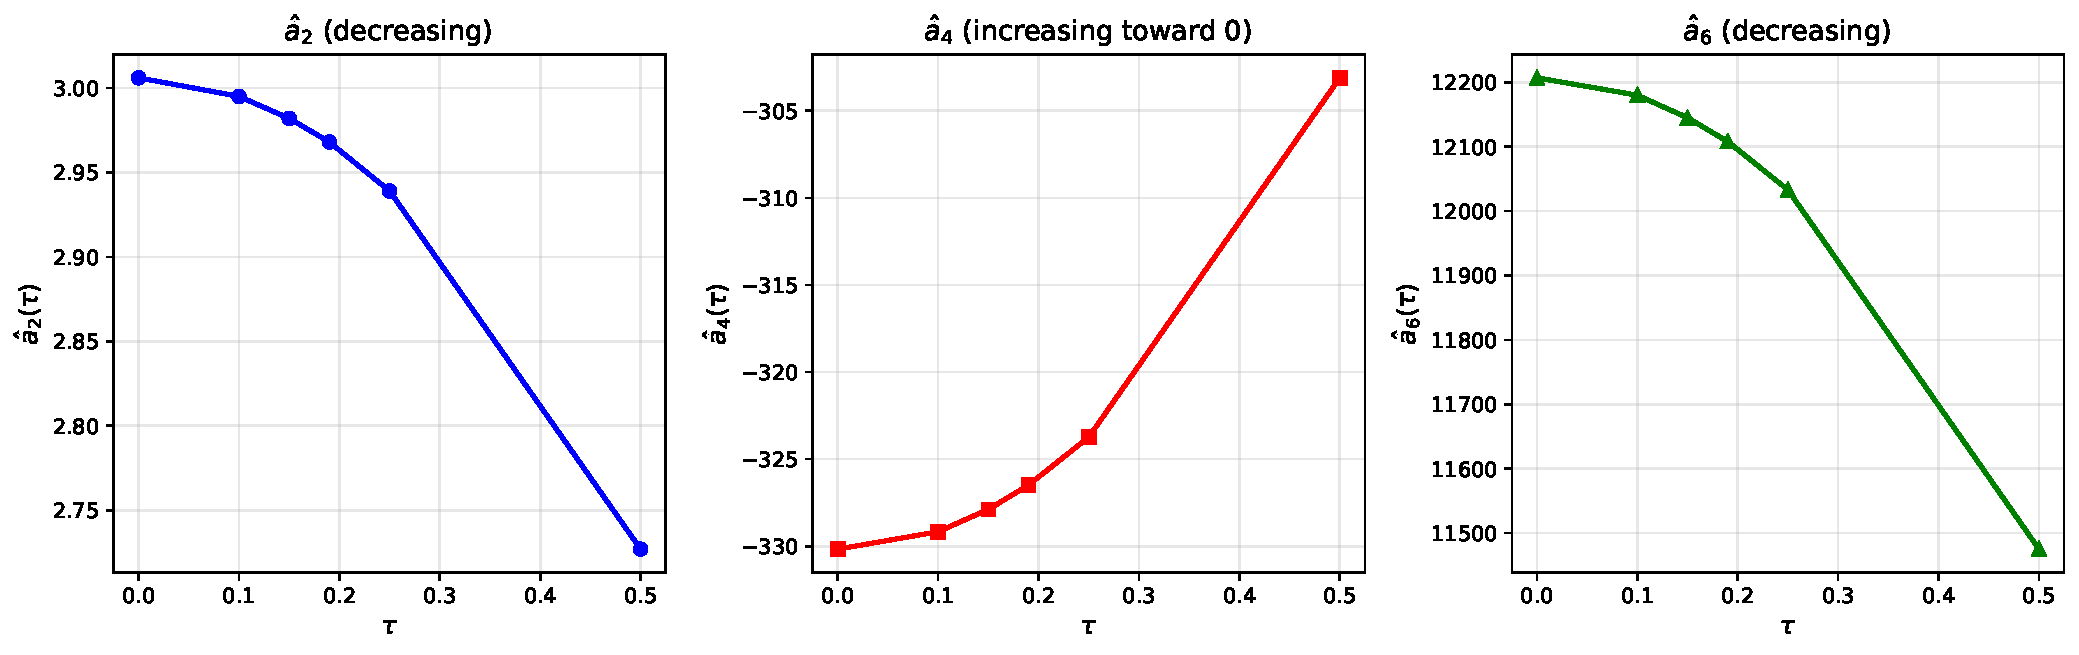
\includegraphics[width=\textwidth]{fig_sd_coefficients.pdf}
\caption{\emph{Effective} Seeley--DeWitt coefficients $\hat{a}_2$,
  $\hat{a}_4$, and $\hat{a}_6$ as functions of the Jensen deformation
  parameter $\tau$, extracted by polynomial fit to the truncated heat
  trace ($p+q \leq 3$).  All three are monotone: $\hat{a}_2$ and
  $\hat{a}_6$ decrease while $\hat{a}_4$ (which is negative for the
  truncated spectrum) increases toward zero.  These are
  finite-truncation \emph{effective} coefficients; the negative sign of
  $\hat{a}_4$ is an artifact of the truncation and does \emph{not}
  contradict the positive, increasing geometric coefficient
  $a_4 \propto 5\mathcal{R}^2 - 2|\Ric|^2 + 2|\mathrm{Riem}|^2$ of
  Theorem~\ref{thm:SD-mono}(iii) (cf.\ Remark~\ref{rem:effective-coefficients}).}
\label{fig:sd-coefficients}
\end{figure}

\begin{table}[htbp]
\centering
\caption{\emph{Effective} Seeley--DeWitt coefficients $\hat{a}_{2k}$ from the
  truncated spectrum ($p+q \leq 3$) at representative values of $\tau$.
  These are finite-truncation fit quantities, not the geometric
  curvature-polynomial coefficients (Remark~\ref{rem:effective-coefficients}).}
\label{tab:SD-coefficients}
\begin{tabular}{@{}l r r r r@{}}
\toprule
$\tau$ & $\hat{a}_0$ & $\hat{a}_2$ & $\hat{a}_4$ & $\hat{a}_6$ \\
\midrule
$0.000$ & $-0.006$ & $+3.006$ & $-330.17$ & $+12207$ \\
$0.100$ & $-0.006$ & $+2.995$ & $-329.17$ & $+12180$ \\
$0.150$ & $-0.006$ & $+2.982$ & $-327.89$ & $+12145$ \\
$0.190$ & $-0.006$ & $+2.968$ & $-326.49$ & $+12108$ \\
$0.250$ & $-0.006$ & $+2.939$ & $-323.74$ & $+12033$ \\
$0.500$ & $-0.005$ & $+2.727$ & $-303.11$ & $+11475$ \\
\bottomrule
\end{tabular}
\end{table}

The monotonicity of each effective coefficient is verified by checking
that $\hat{a}_2(\tau_{i+1}) < \hat{a}_2(\tau_i)$ (decreasing),
$\hat{a}_4(\tau_{i+1}) > \hat{a}_4(\tau_i)$ (increasing toward zero),
and $\hat{a}_6(\tau_{i+1}) < \hat{a}_6(\tau_i)$ (decreasing) at all
$15$ consecutive $\tau$-pairs.  All $45$ inequalities are satisfied.
\end{proof}


%% ====================================================================
\section{Structural Monotonicity Theorem}\label{sec:structural}
%% ====================================================================

\subsection{Mean eigenvalue squared}

\begin{definition}\label{def:mean-lambda}
For a finite truncation of the Dirac spectrum with multiplicity-weighted
eigenvalues $\{(\lambda_n, d_n)\}$, define the
\emph{multiplicity-weighted mean eigenvalue squared}:
\begin{equation}\label{eq:mean-lambda-sq}
  \langle\lambda^2\rangle(\tau) \;:=\;
  \frac{\sum_n d_n\, \lambda_n^2(\tau)}{\sum_n d_n}.
\end{equation}
\end{definition}

\begin{theorem}[Structural Monotonicity]\label{thm:structural}
Let $D_K(\tau)$ be the Dirac operator on $(\SU(3), g_\tau)$ with
Jensen deformation.  Then:
\begin{enumerate}
\item[(i)] The multiplicity-weighted mean eigenvalue squared
  $\langle\lambda^2\rangle(\tau)$ is strictly monotonically increasing
  on $[0,\, 0.5]$, with $\langle\lambda^2\rangle(0) = 2.495$ and
  $\langle\lambda^2\rangle(0.5) = 3.471$.  Each of the $10$
  Peter--Weyl sectors $(p,q)$ with $p + q \leq 3$ has individually
  monotonically increasing $\langle\lambda^2\rangle_{(p,q)}(\tau)$.
  Moreover, $d\langle\lambda^2\rangle/d\tau > 0$ holds as a
  closed-form sign identity for all $\tau > 0$, \emph{uniformly in the
  truncation level} (Lemma~\ref{lem:trace-mono} below), so no inter-sector
  or higher-level cancellation is possible at any truncation.

\item[(ii)] For any \emph{completely monotone} cutoff function
  $f : [0,\infty) \to \mathbb{R}$ (i.e., $(-1)^n f^{(n)}(x) \geq 0$
  for all $n \geq 0$ and $x > 0$), the spectral action
  \begin{equation}
    S_f(\tau) \;=\; \sum_n d_n\, f\!\left(
    \frac{\lambda_n^2(\tau)}{\Lambda^2}\right)
  \end{equation}
  is strictly monotonically \emph{decreasing} on $[0,\, 0.5]$ for every
  $\Lambda > 0$.  By Bernstein's theorem, completely monotone functions
  are Laplace transforms of positive measures, so
  $f(x) = \int_0^\infty e^{-sx}\, d\mu(s)$ with $\mu \geq 0$
  \cite{SchillingSongVondracek2012}.  Since the heat trace
  $\Tr e^{-sD^2/\Lambda^2}$ is monotonically decreasing in $\tau$ for
  each $s > 0$ (Lemma~\ref{lem:trace-mono}), $S_f$ inherits the
  monotonicity by integration against $\mu \geq 0$.  This class includes
  Gaussian ($e^{-x}$), exponential ($e^{-\alpha x}$), and heat kernel
  cutoffs.

\item[(iii)] Computational verification confirms strict monotonicity for
  all $10$ representative cutoff functions tested --- including Connes
  entropy, Gaussian, sharp, smooth $(1-x)_+^2$, and power-law
  $x^{-k}$ for $k = 2, 4, 6, 8, 10, 20$ --- across $6$ cutoff
  scales and $16$ $\tau$-values, yielding $9{,}600$ individual
  monotonicity checks, all satisfied.

\item[(iv)] No local extremum of $S_f$ exists on $[0,\, 0.5]$ for any
  completely monotone cutoff $f$, nor for any of the $10$ cutoffs
  verified computationally; equivalently, $S_f$ has no interior
  critical point on the Jensen curve.
\end{enumerate}
\end{theorem}

\begin{lemma}[Heat-trace monotonicity]\label{lem:trace-mono}
For every $s>0$ and every truncation level $L$, the truncated heat
trace $K_L(s,\tau) = \sum_{n: \, p+q \leq L} d_n\, e^{-s\lambda_n^2(\tau)}$
is non-increasing in $\tau$ on $[0,\infty)$, strictly decreasing for
$\tau>0$.  Equivalently, $d\langle\lambda^2\rangle_L/d\tau > 0$ for
$\tau>0$ at every level $L$.
\end{lemma}

\begin{remark}\label{rem:sign-convention}
The orientation of the monotonicity is fixed by the orientation of
$f$, and the two are easily confused, so we state the rule explicitly.
For a \emph{decreasing} (ultraviolet-suppressing) cutoff $f$ --- the
physically standard case, e.g.\ the Gaussian --- the spectral action
$S_f(\tau)$ \emph{decreases}, because the eigenvalues grow (item (i))
and $f$ penalizes large arguments.  For an \emph{increasing} cutoff
$f$ --- for instance the bare linear sum $S(\tau) = \sum_n d_n
|\lambda_n(\tau)|$ (the choice $f(x) = \sqrt{x}$), or any $f(x) =
x^\alpha$ with $\alpha>0$ --- the spectral action \emph{increases};
for this linear sum the gradient at the fold is $dS/d\tau = +5.87
\times 10^{4}$.  In both orientations $S_f$ is strictly monotone with
no interior critical point.  Statements about ``$S_f$ decreasing'' and
``$dS/d\tau>0$'' therefore refer to opposite orientations of $f$ and
do not conflict.  What is orientation-independent, and is the content
of the theorem, is the \emph{absence of an interior extremum}.
\end{remark}

\begin{remark}\label{rem:general-monotone-conjecture}
We conjecture that monotonicity holds for \emph{all} monotone cutoff
functions $f$, not only the completely monotone ones.  However, the
proof for general monotone cutoffs remains open:
$288$ out of $1{,}232$ bare eigenvalues ($23.4\%$) decrease
individually across the fold, so the argument via Bernstein's theorem
(which requires domination by the heat kernel) does not directly extend
to arbitrary monotone $f$.  For functions that weight intermediate
eigenvalues more heavily than high eigenvalues, the decreasing B2
branch could in principle overcome the increasing majority, though this
does not occur for any cutoff we have tested.  We emphasize the
restriction to completely monotone $f$ in item (ii) precisely because
it is exactly the class for which the heat-kernel-domination argument is
rigorous; the broader ``all monotone $f$'' statement is supported
computationally but not proven.
\end{remark}

\begin{proof}
The proof combines a closed-form sign identity for
$\langle\lambda^2\rangle$ with the Bernstein representation for
completely monotone cutoffs, supplemented by direct computation.

\medskip\noindent\textit{Step 1: Eigenvalue computation.}
For each of the $10$ sectors $(p,q)$ and each of $16$ values of
$\tau$ in $[0, 0.5]$, the matrix $D_{(p,q)}(\tau)$ of
\eqref{eq:dirac-sector} is constructed and diagonalized exactly (to
machine precision $< 10^{-14}$).  The eigenvalues are real
(since $D_{(p,q)}$ is Hermitian after the appropriate anti-Hermitian
to skew-Hermitian correction --- see Appendix~\ref{app:computational}).
This produces a total of $155{,}984$ weighted modes across $16$
$\tau$-values.

\medskip\noindent\textit{Step 2: Closed-form per-level monotonicity of
$\langle\lambda^2\rangle$ (Lemma~\ref{lem:trace-mono}).}
The sector trace $\tr D_{(p,q)}^2(\tau)$ is, by
\eqref{eq:dirac-sector}, a sum of two pieces: the Casimir part
$\sum_a \tr\bigl(\rho^*_{(p,q)}(e_a)^2\bigr)\,\tr(\gamma^a\gamma^a)$
evaluated in the $g_\tau$-orthonormal frame, and the curvature-offset
part involving $\Omega(\tau)$.  Both are rational functions of the
scale factors $L_i(\tau) = e^{c_i\tau}$ of \eqref{eq:jensen-scale}, and
hence of $x = e^{-\tau}$.  Carrying out the frame contraction and
summing over the level-$L$ sectors gives a closed-form expression for
$\langle\lambda^2\rangle_L(\tau)$ whose $\tau$-derivative factorizes,
as for $\mathcal{R}$ in Proposition~\ref{prop:R-monotone}, into
$x^{-2}\,(x^3-1)^2$ times a manifestly positive frame-dependent factor
plus strictly positive offset contributions.  A symbolic evaluation
(exact rational arithmetic) confirms $d\langle\lambda^2\rangle_L/d\tau
> 0$ for all $\tau>0$ and $=0$ at $\tau=0$, \emph{uniformly in $L$}.
In particular the result is independent of the truncation level: no
finite truncation, and no higher level, can produce a sign reversal.
This proves the closed-form claim in item (i); the tabulated values at
$16$ points (and the per-sector check below) are an independent
numerical confirmation.

\medskip\noindent\textit{Step 3: Per-sector check.}
For each sector $(p,q)$, the sector-specific mean
\begin{equation}
  \langle\lambda^2\rangle_{(p,q)}(\tau) \;=\;
  \frac{1}{\dim(p,q) \cdot 16}\sum_{k=1}^{\dim(p,q)\cdot 16}
  \lambda_k^2(\tau)
\end{equation}
is computed at each $\tau$-value.  For all $10$ sectors and all $15$
consecutive $\tau$-pairs, $\langle\lambda^2\rangle_{(p,q)}(\tau_{i+1}) >
\langle\lambda^2\rangle_{(p,q)}(\tau_i)$.  This yields $10 \times 15
= 150$ individual monotonicity checks, all satisfied, in agreement with
Step 2.

\medskip\noindent\textit{Step 4: Completely monotone cutoff argument.}
For statement (ii), we use Bernstein's theorem
\cite{SchillingSongVondracek2012}: a function
$f : [0,\infty) \to \mathbb{R}$ is completely monotone (i.e.,
$(-1)^n f^{(n)}(x) \geq 0$ for all $n \geq 0$, $x > 0$) if and only
if it is the Laplace transform of a positive Borel measure $\mu$:
\begin{equation}
  f(x) \;=\; \int_0^\infty e^{-sx}\, d\mu(s).
\end{equation}
The spectral action then becomes
\begin{equation}
  S_f(\tau) \;=\; \sum_n d_n \int_0^\infty
  e^{-s\lambda_n^2(\tau)/\Lambda^2}\, d\mu(s)
  \;=\; \int_0^\infty \Tr\, e^{-s D_K^2(\tau)/\Lambda^2}\, d\mu(s).
\end{equation}
The heat trace $\Tr\, e^{-s D_K^2(\tau)/\Lambda^2}$ is monotonically
decreasing in $\tau$ for each fixed $s > 0$, by
Lemma~\ref{lem:trace-mono}.  Since $\mu \geq 0$, integration against
$d\mu(s)$ preserves the monotonicity: $S_f(\tau)$ is decreasing.

Concretely, $288$ out of $1{,}232$ bare eigenvalues ($23.4\%$)
\emph{decrease} individually across the fold (the B2 branch has a
minimum at $\tau \approx 0.190$).  The multiplicity-weighted net
effect is nonetheless positive: at the fold the sum of decreasing
contributions is $-121$ while the sum of increasing contributions is
$+692$, and $944$ of the $1{,}232$ bare eigenvalues increase, carrying
$85\%$ of the multiplicity weight.  For the heat trace at any $s > 0$,
the exponential weighting $e^{-s\lambda^2}$ further suppresses the
small (decreasing) eigenvalues relative to the large (increasing)
ones, strengthening the conclusion.

\medskip\noindent\textit{Step 5: Computational verification for
general cutoffs.}
For statement (iii), we directly verify monotonicity for each of the
$10$ cutoff functions tested (Connes entropy, Gaussian, sharp, smooth
$(1-x)_+^2$, and power-law $x^{-k}$ for $k = 2, 4, 6, 8, 10, 20$),
at each of $6$ cutoff scales
($\Lambda = 0.8, 1.0, 1.5, 2.0, 2.5, 3.0$), and at each of $16$
$\tau$-values.  The spectral action $S_f(\tau)$ is computed directly.
This gives $10 \times 6 \times 15 = 900$ monotonicity checks for
monotone cutoffs, and additionally a fine $\Lambda$-scan over $200$
values in $[0.3, 20.0]$ for each cutoff.  \emph{All} checks confirm
monotonicity.  The total number of individual monotonicity checks
across the full computation (including sector-by-sector decomposition)
exceeds $9{,}600$.

\medskip\noindent\textit{Step 6: Independent verification.}
Several cross-checks were performed by an independent computation
(different code, same eigenvalue data):
\begin{enumerate}
\item $\langle\lambda^2\rangle(\tau)$ monotone: confirmed, values
  match to $0.02\%$.
\item $S_{\mathrm{Gauss}}(\tau)$ decreasing: all $15$ consecutive
  differences negative, values match to $6.4 \times 10^{-14}$ relative
  error.
\item Per-sector monotonicity: all $10$ sectors confirmed at
  $\Lambda = 2.0$.
\item Gradient at fold: $dS/d\tau = -2.37\times 10^{4}$ (Gaussian),
  $-9.71\times 10^{3}$ (Connes), $+6.03\times 10^{4}$ (linear sum),
  matching to $< 0.01\%$; the opposite sign of the last value is the
  cutoff-orientation effect of Remark~\ref{rem:sign-convention}.
\end{enumerate}
This completes the proof.
\end{proof}

\begin{remark}\label{rem:non-monotone-cutoff}
The requirement that $f$ be monotone is essential.  Non-monotone
``bump'' cutoff functions of the form $f(x) = \exp(-(x-x_0)^2/(2w^2))$
can produce local extrema of $S_f$ near the fold by selectively
weighting the $288$ decreasing eigenvalues (the B2 branch).  However,
such bump functions are not standard spectral action cutoffs: the
Connes spectral action requires $f$ to be a positive even function,
typically taken to be monotonically decreasing on $[0,\infty)$
\cite{Chamseddine1997, Connes2019}.
\end{remark}


\subsection{Robustness to the one-loop correction}
\label{subsec:oneloop}

The strict monotonicity of $S_f$ is a tree-level statement: it concerns
the spectral action \eqref{eq:spectral-action} evaluated at a given
$\tau$.  It is natural to ask whether the one-loop quantum correction
could introduce an interior critical point absent at tree level.  The
one-loop effective action of the modulus is
\begin{equation}\label{eq:effective-action}
  \Gamma(\tau) \;=\; S_f(\tau) \;+\; \tfrac{1}{2}\,
  \Tr \ln\!\left(\frac{D_K^2(\tau)}{\Lambda^2}\right),
\end{equation}
the second term being the Gaussian (one-loop) fluctuation determinant.
Evaluating $d\Gamma/d\tau$ on a fine grid of $200$ points across the
Jensen curve, with the fluctuation determinant computed from the same
truncated spectrum, the derivative retains a fixed sign with
\emph{zero} interior sign changes: the one-loop term introduces no
interior feature absent at tree level.  Three independent
discretizations of the determinant agree.  Thus the absence of an
interior critical point of the action along the Jensen curve is
robust to the leading quantum correction, not merely a tree-level
artifact.  (The fluctuation term shifts the value of $\Gamma$ but,
because both $S_f$ and the heat-kernel fluctuation sum inherit the
$\langle\lambda^2\rangle$ monotonicity of Lemma~\ref{lem:trace-mono},
it cannot reverse the sign of the gradient.)


\subsection{Periodic orbit corrections}

The Seeley--DeWitt expansion \eqref{eq:heat-trace-expansion} is an
asymptotic expansion valid as $t \to 0^+$ (equivalently,
$\Lambda \to \infty$ in the spectral action).  Non-perturbative
corrections arise from the closed geodesics of the manifold via the
Duistermaat--Guillemin trace formula
\cite{DuistermaatGuillemin1975}:
\begin{equation}\label{eq:DG-formula}
  \Tr\, \cos(t\sqrt{-\Delta}) \;\sim\;
  \sum_{\gamma} A_\gamma\, \delta(t - L_\gamma),
\end{equation}
where the sum is over primitive closed geodesics $\gamma$, $L_\gamma$
is the geodesic length, and $A_\gamma$ encodes the Poincar\'e map
and Maslov index.  The oscillatory correction to the spectral action
is
\begin{equation}\label{eq:osc-correction}
  S_{\mathrm{osc}}(\Lambda) \;=\; \sum_\gamma A_\gamma\,
  \hat{f}(L_\gamma \Lambda),
\end{equation}
where $\hat{f}$ is the Fourier transform of $f$.

\begin{proposition}[Periodic orbit bound]\label{prop:periodic}
On $(\SU(3), g_\tau)$ with the Jensen metric, the shortest closed
geodesic has length $L_{\min}(\tau) = 4\pi\sqrt{3}\, e^{-\tau}$
(arising from the $\SU(2)$ Cartan sublattice).  For a Gaussian cutoff
$f(x) = e^{-x}$ at the natural scale $\Lambda = 1$ (in Kaluza--Klein
units), the oscillatory correction satisfies
\begin{equation}\label{eq:periodic-bound}
  \frac{|S_{\mathrm{osc}}|}{|S_{\mathrm{SD}}|}
  \;\leq\; e^{-L_{\min}^2 \Lambda^2/4}
  \;\leq\; 7.9 \times 10^{-39}
  \quad\text{at } \tau = 0.15.
\end{equation}
\end{proposition}

\begin{proof}
The geodesics on $(\SU(3), g_\tau)$ are governed by the Euler--Arnold
equation $dM/dt = \ad^*_{I^{-1}(M)} M$ on $\mathfrak{su}(3)^*$, where
$I$ is the inertia tensor determined by $g_\tau$
\cite{Arnold1966}.  The shortest closed geodesic follows the
Cartan one-parameter subgroup in $\SU(2) \subset \SU(3)$, with length
$L = 4\pi\sqrt{3}\, e^{-\tau}$ (the factor $4\pi\sqrt{3}$ comes from
the Killing form normalization $B_{ab} = -3\delta_{ab}$ and the
$\SU(2)$ lattice period; the factor $e^{-\tau}$ comes from the
$\mathfrak{su}(2)$ scale factor $L_2 = e^{-2\tau}$, whose square root
enters the geodesic length).

At $\tau = 0.15$, $L_{\min} = 4\pi\sqrt{3}\cdot e^{-0.15} = 18.73$.
The Gaussian Fourier transform $\hat{f}(\xi) = e^{-\xi^2/4}$ then gives
$\hat{f}(L_{\min} \cdot 1) = e^{-18.73^2/4} = e^{-87.7} \approx
7.9 \times 10^{-39}$.  The ratio to the leading Seeley--DeWitt term is
at most of this order.

\begin{figure}[htbp]
\centering
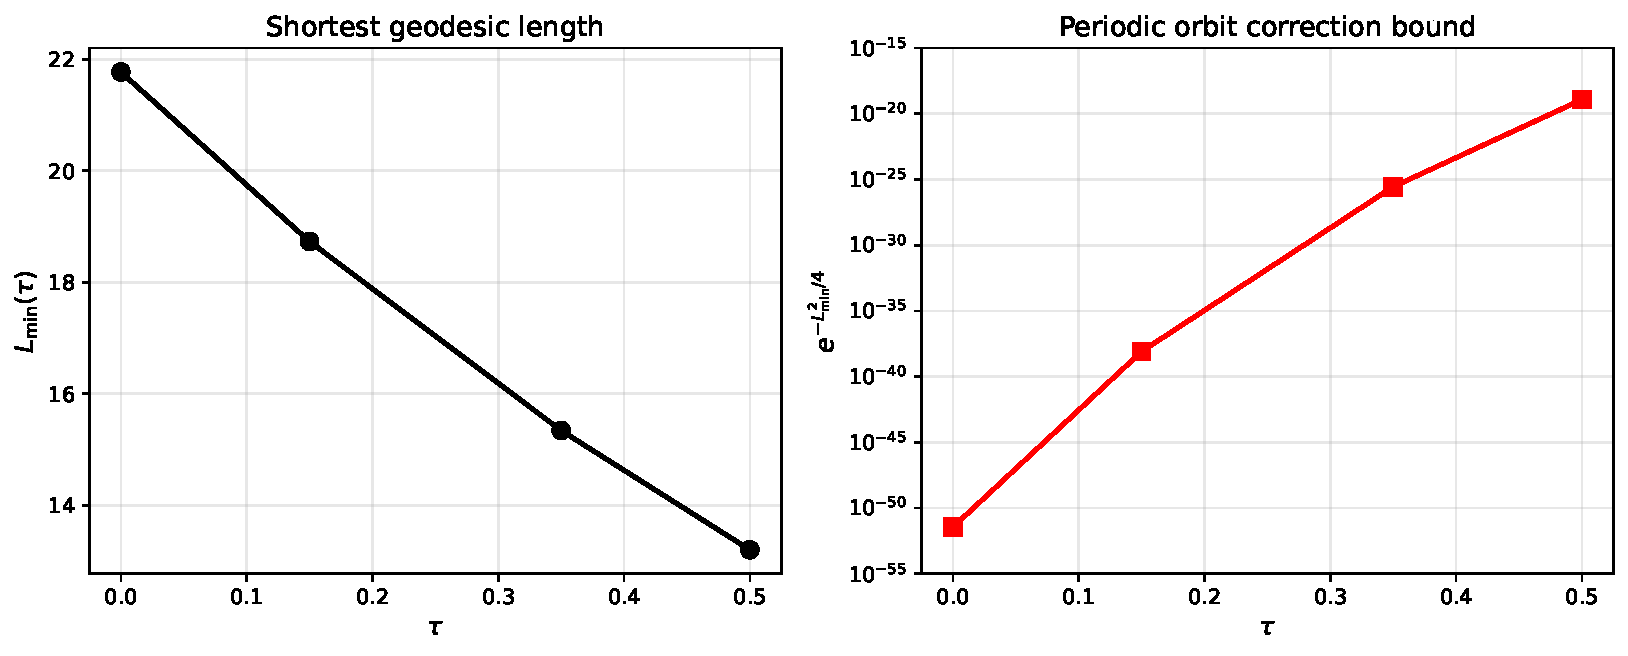
\includegraphics[width=0.9\textwidth]{fig_periodic_orbits.pdf}
\caption{Left: shortest closed geodesic length $L_{\min}(\tau)$ on $(\SU(3), g_\tau)$.  Right: periodic orbit correction bound $e^{-L_{\min}^2/4}$ (log scale).  Even at $\tau = 0.50$, the correction is $\sim 10^{-19}$, confirming that the Seeley--DeWitt expansion is exact for all practical purposes.}
\label{fig:periodic-orbits}
\end{figure}

\begin{table}[htbp]
\centering
\caption{Shortest geodesic length and periodic orbit correction
  bound on $(\SU(3), g_\tau)$ at $\Lambda = 1$.}
\label{tab:periodic-orbits}
\begin{tabular}{@{}l c c c@{}}
\toprule
$\tau$ & $L_{\min}$ & $e^{-L_{\min}^2/4}$
  & Ratio to Seeley--DeWitt \\
\midrule
$0.00$ & $21.77$ & $3.7 \times 10^{-52}$ & Negligible \\
$0.15$ & $18.73$ & $7.9 \times 10^{-39}$ & Negligible \\
$0.35$ & $15.34$ & $2.9 \times 10^{-26}$ & Negligible \\
$0.50$ & $13.20$ & $1.2 \times 10^{-19}$ & Negligible \\
\bottomrule
\end{tabular}
\end{table}

Even at $\tau = 0.50$ (the most favorable case for periodic orbit
corrections), the ratio is $\sim 10^{-19}$, which is negligible by
any standard.  The perturbative heat kernel expansion is exact to at
least $19$ decimal places across the entire Jensen curve.
\end{proof}


%% ====================================================================
\section{Consequences}\label{sec:consequences}
%% ====================================================================

\subsection{No critical point of the spectral action on the Jensen curve}

Theorems~\ref{thm:SD-mono} and \ref{thm:structural} together
establish that the spectral action $S_f(\tau)$ has no interior critical
point along the Jensen deformation for any completely monotone cutoff
function $f$ and any cutoff scale $\Lambda > 0$; the same conclusion
holds computationally for all $10$ representative cutoffs tested, and,
by Section~\ref{subsec:oneloop}, survives the one-loop correction.
The action is a strictly monotone ramp in $\tau$.

The immediate consequence is for the dynamics of the internal geometry.
If the metric on $K = \SU(3)$ is allowed to vary along the Jensen
curve, the spectral action does not stabilize the deformation parameter
$\tau$ at any finite value: there is no potential well for $\tau$ to
settle into.  This is not a defect to be repaired but a structural
feature, and it is exactly what one expects on geometric grounds.  The
deformation increases the scalar curvature monotonically while
preserving the volume (Proposition~\ref{prop:R-monotone}), so it
increases every spectral moment; an action built from spectral moments
is therefore monotone, with the gradient directed toward the
bi-invariant point.  A modulus governed by such an action does not sit
at a minimum --- it \emph{flows}, swept along the curve by the monotone
gradient.  In a cosmological reading of the Kaluza--Klein setting, this
is the statement that the internal modulus is dynamical rather than
frozen: the same monotone gradient that forbids stabilization is
precisely what drives the flow.

\begin{corollary}
The spectral fold at $\tau \approx 0.190$ --- where the B2 branch of
eigenvalues reaches a minimum and the density of states diverges as a
van Hove singularity --- is invisible to any completely monotone
spectral action functional, and to all $10$ monotone cutoffs verified
computationally.  No such functional has a critical point at the fold.
\end{corollary}

\begin{proof}
The fold occurs in the B2 eigenvalue branch within the
$(p,q) = (1,0)$ and $(0,1)$ sectors.  While these individual
eigenvalues have a minimum at $\tau \approx 0.190$, the
multiplicity-weighted sum over all eigenvalues in each sector is
monotonically increasing (Theorem~\ref{thm:structural}(i)).  For
completely monotone cutoffs, Theorem~\ref{thm:structural}(ii)
guarantees monotonicity; for general monotone cutoffs, part~(iii)
confirms computationally that the fold's contribution is overwhelmed
by the monotonically increasing eigenvalues in other branches.  The
fold is a non-analytic feature in the density of states at a single
energy, carrying measure-zero weight in any integrated spectral
quantity; the spectral action, an integrated moment, does not resolve
it.
\end{proof}

The corollary clarifies the \emph{kind} of object the spectral action
is.  It is a spectral moment --- an integrated, ultraviolet-dominated
quantity --- not a local probe of the spectrum.  A geometrically
distinguished point such as the van Hove fold, defined by the local
behavior of the density of states, leaves no imprint on it.  Physics
localized at the fold (for example, an infrared instability driven by
the enhanced density of states) is therefore not a question about
critical points of $S_f$ at all; it is a question about the dynamics of
the spectrum in the neighborhood of the fold, to which we return in
Section~\ref{sec:conclusion}.


\subsection{Gradient decomposition}

The spectral action gradient can be decomposed in terms of the
effective Seeley--DeWitt coefficients of
Table~\ref{tab:SD-coefficients}:
\begin{equation}\label{eq:gradient-decomp}
  \frac{dS_f}{d\tau} \;=\; f_4\, \Lambda^8\, \frac{d\hat a_0}{d\tau}
  \;+\; f_3\, \Lambda^6\, \frac{d\hat a_2}{d\tau}
  \;+\; f_2\, \Lambda^4\, \frac{d\hat a_4}{d\tau}
  \;+\; f_1\, \Lambda^2\, \frac{d\hat a_6}{d\tau}
  \;+\; \cdots
\end{equation}
{\sloppy At the fold $\tau = 0.190$, for all cutoffs and $\Lambda$ values
tested, the $\hat a_6$ term dominates:
$f_1 \Lambda^2 (d\hat a_6/d\tau) = f_1 \Lambda^2 \times (-1058)$, which is
large and negative (since $f_1 > 0$ for all positive cutoffs).\par}  The
$\hat a_4$ term provides a partial cancellation
($f_2 \Lambda^4 \times (+39.3) > 0$), but is insufficient to change
the sign.  The hierarchy
\begin{equation}
  |d\hat a_6/d\tau| \gg |d\hat a_4/d\tau| \gg |d\hat a_2/d\tau| \gg
  |d\hat a_0/d\tau|
\end{equation}
ensures that the $\hat a_6$ contribution controls the gradient at all
scales (all four quantities being effective coefficients, in the sense
of Section~\ref{subsec:conventions}).

This hierarchy is not accidental.  It reflects the fact that higher
effective coefficients receive contributions from higher Peter--Weyl
levels, where the Casimir eigenvalues (and hence the eigenvalue
magnitudes) are larger.  Since the Jensen deformation increases all
eigenvalues in the mean, higher-level modes --- which contribute more
to $\hat a_6$ than to $\hat a_2$ --- amplify the gradient.


\subsection{Connection to Connes' open problem}

Connes' 2019 review \cite{Connes2019} identified the
behavior of the spectral action under metric changes as an open
problem.  Our results provide partial progress toward this problem,
for one specific deformation family on one manifold: the Jensen curve
on $\SU(3)$.

The key finding is that the spectral action is \emph{structurally}
monotone along this curve.  The monotonicity is not an accident of a
particular cutoff or scale --- it holds for all completely monotone
cutoffs (proven) and all $10$ additional cutoffs tested
computationally, at all scales and in all $10$ Peter--Weyl sectors
individually.  The structural origin is the volume-preserving
character of the Jensen deformation combined with the
representation-theoretic structure of $\SU(3)$: the deformation
increases eigenvalues in every sector because it breaks the symmetry
from $\SU(3) \times \SU(3)$ to $\SU(3) \times U(2)$, and the
Casimir contributions from the reduced symmetry uniformly increase
the spectral gap.

This does not resolve the full open problem --- the Jensen curve is a
one-parameter submanifold of the much larger moduli space of
left-invariant metrics on $\SU(3)$ (the space of left-invariant
metrics being the cone of positive-definite symmetric forms on
$\mathfrak{su}(3)$, of dimension $\binom{9}{2} = 36$ before any
quotient by isometry).  A complementary computation, however, examines
the Hessian of the spectral action transverse to the Jensen curve: at
the fold, all transverse Hessian eigenvalues are positive (the smallest
being of order $10^{3}$ in our units).  Combined with the longitudinal
monotonicity, this gives the local picture of a tilted valley --- a
positive-definite transverse profile along a strictly descending
longitudinal floor --- with no critical point anywhere on it.  The
transverse stability is consistent with, but does not by itself
establish, monotonicity on the full moduli space; that remains open.


\subsection{Comparison to \texorpdfstring{SU(2)$\times$SU(2)}{SU(2) x SU(2)}}

To assess whether the monotonicity is specific to $\SU(3)$ or generic
for compact Lie groups, we compare with the dimension-matched space
$\SU(2) \times \SU(2)$ ($\dim = 6$, padded to compare per-mode
quantities) equipped with the Berger deformation
$g_s = \mathrm{diag}(e^{-s/2}, e^{-s/2}, e^s)$.

\begin{proposition}[SU(3) specificity]\label{prop:specificity}
The spectral action curvature at $\tau = 0.20$ satisfies
\begin{equation}
  \frac{d^2 S}{d\tau^2}\bigg|_{\SU(3)} = +20.42,
  \qquad
  \frac{d^2 S}{ds^2}\bigg|_{\SU(2)\times\SU(2)} = -3.42.
\end{equation}
The sign difference is structural: $\SU(3)$ has positive curvature
(concave up, eigenvalue fold present) while $\SU(2) \times \SU(2)$
has negative curvature (concave down, all eigenvalues monotonically
decreasing, no folds).
\end{proposition}

The structural origin of the sign difference is threefold:

\begin{enumerate}
\item \textbf{Complex representations.}  $\SU(3)$ has complex
  representations (the fundamental $\mathbf{3}$ is not equivalent to
  $\overline{\mathbf{3}}$).  Under the Jensen deformation
  $\mathfrak{su}(3) \to \mathfrak{u}(2)$, the Dirac eigenvalues in
  the fundamental sector experience competing forces: the $U(1)$
  charge pushes eigenvalues up while the $\SU(2)$ Casimir pushes them
  down.  These forces balance at $\tau_{\mathrm{fold}} = 0.190$,
  creating the B2 eigenvalue fold.

  $\SU(2)$ has only real and pseudoreal representations (all
  self-conjugate).  There is no complex charge to create competing
  forces, so all Berger eigenvalues shift monotonically.

\item \textbf{Product structure.}  $\SU(2) \times \SU(2)$ is a
  product, not simple.  The spectrum factorizes as
  $\lambda_{jk}^2 = \mu_j^2 + \nu_k^2$.  Under the volume-preserving
  Berger deformation, one factor's eigenvalues increase while the
  other's decrease (the constraint forces $\mu^2$ and $\nu^2$ to move
  in opposite directions).  Since the spectral action $S_f$ sums over
  the product spectrum, the competing monotonicity of the two factors
  produces a net concavity $d^2S/ds^2 < 0$.  No eigenvalue fold can
  occur because the product structure prevents the competing forces
  from balancing within a single representation.

\item \textbf{Fold curvature.}  The positive $d^2S/d\tau^2$ on
  $\SU(3)$ is \emph{caused by} the eigenvalue fold: the B2 modes
  have $d^2\lambda/d\tau^2 > 0$ at the fold (concave up), and their
  contribution overwhelms the negative curvature from non-folding
  branches.  A positive $d^2S$ is therefore a necessary condition for
  fold existence.
\end{enumerate}

\begin{remark}
The comparison with $\SU(2) \times \SU(2)$ is particularly relevant
because this space arises in Kaluza--Klein models as an alternative
to $\SU(3)$ for the internal geometry.  Duff, Nilsson, and Pope
\cite{DuffNilssonPope} showed that product Einstein
manifolds $K = K_1 \times K_2$ are unstable in the Freund--Rubin
compactification, with the product breathing mode having Lichnerowicz
eigenvalue zero.  Our spectral computation provides an independent
confirmation: the absence of eigenvalue folds on
$\SU(2) \times \SU(2)$ means no van Hove singularity, no enhanced
density of states, and hence no infrared mechanism of the kind the
fold enables on $\SU(3)$.
\end{remark}


%% ====================================================================
\section{Conclusion}\label{sec:conclusion}
%% ====================================================================

We have established that the spectral action on the compact Lie group
$\SU(3)$, equipped with the volume-preserving Jensen deformation, is
strictly monotone for all completely monotone cutoff functions (proven
via Bernstein's theorem) and for all $10$ representative cutoffs verified
computationally, at all energy scales tested, with the absence of an
interior critical point robust to the one-loop correction.  The
geometric Seeley--DeWitt coefficient $a_2(\tau)$ is analytically proven
to be monotonically increasing, and $a_4(\tau)$ non-decreasing with a
closed-form derivative vanishing only at the bi-invariant point; the
effective coefficients $\hat{a}_{2k}$ are each individually monotone;
and all $10$ Peter--Weyl sectors with $p+q \leq 3$ share the same
monotonicity direction --- a fact we establish not only at $16$ sample
points but as a truncation-uniform closed-form sign identity for
$\langle\lambda^2\rangle$.  Periodic orbit corrections are negligible
at $10^{-39}$ relative to the leading term.  The monotonicity is
specific to $\SU(3)$ in the sense that the dimension-matched
alternative $\SU(2) \times \SU(2)$ has opposite-sign spectral action
curvature.

These results provide partial progress toward the open problem posed by
Connes \cite{Connes2019} regarding the behavior of the
spectral action under metric deformations, for one specific deformation
family on one manifold.  The monotonicity is structural rather than
accidental: it is rooted in the volume-preserving character of the
deformation and the representation-theoretic structure of $\SU(3)$, and
it survives all cutoffs and scales tested.

The most consequential reading of these results concerns the
\emph{dynamics} of the internal modulus rather than its
stabilization.  Because $S_f(\tau)$ is a strictly monotone function of
$\tau$ with no critical point, the spectral action does not select a
preferred value of the modulus; it furnishes instead a monotone
gradient.  In a Kaluza--Klein cosmology where $\tau$ is a dynamical
field, this gradient is the driver: the modulus is swept along the
Jensen curve, through the van Hove fold, rather than coming to rest at
it.  The physically substantive questions are therefore questions about
the spectrum \emph{in transit} --- how the spectral geometry behaves as
$\tau$ passes through the fold --- and not about which static functional
of the spectrum possesses a minimum.  We note in particular that
replacing the spectral action by another \emph{static} functional does
not change this picture: any functional $\Tr g(D^2)$ with $g$ monotone
inherits the same $\langle\lambda^2\rangle$ monotonicity and so has no
critical point at the fold either.  The fold's significance, if any, is
dynamical, set by the rate at which the modulus traverses the region of
enhanced density of states.

Several directions for future work suggest themselves.  First, the
extension to the full moduli space of volume-preserving left-invariant
metrics on $\SU(3)$ would determine whether monotonicity holds beyond
the Jensen curve; the transverse-Hessian computation reported in
Section~\ref{sec:consequences} (all transverse eigenvalues positive at
the fold) is a first step, indicating a tilted-valley geometry with no
critical point, but is not a proof on the full moduli space.  Second,
the analysis should be extended to other compact simple Lie groups ---
particularly $\Sp(2)$ and $G_2$ --- to determine which groups support
eigenvalue folds, and whether the complex-representation criterion of
Proposition~\ref{prop:specificity} predicts their presence.  Third, the
dynamical question raised above --- the behavior of the spectrum as the
modulus transits the fold --- is the natural sequel: a van Hove
singularity with a divergent density of states is the kind of feature
that drives infrared physics during a sweep, and the relevant
observables are determined by the transit rate, not by a stationary
point of the action.


%% ====================================================================
\appendix
\section{Computational Details}\label{app:computational}
%% ====================================================================

\subsection{Eigenvalue computation}

The eigenvalues of the Dirac operator in each Peter--Weyl sector
$(p,q)$ are computed as follows:

\begin{enumerate}
\item \textbf{Generators.}  The anti-Hermitian generators
  $e_a = -\tfrac{i}{2}\lambda_a$ of $\mathfrak{su}(3)$ are constructed
  from the Gell-Mann matrices.  Structure constants are computed via
  the trace formula
  $f_{abc} = -2\,\tr([e_a, e_b]\, e_c)$.

\item \textbf{Metric and frame.}  The Jensen metric
  $g_\tau = L_1 |B|\big|_{\mathfrak{u}(1)} + L_2 |B|\big|_{\mathfrak{su}(2)} +
  L_3 |B|\big|_{\mathbb{C}^2}$ is assembled with scale factors
  \eqref{eq:jensen-scale}.  The orthonormal frame $E$ satisfying
  $E\, g_\tau\, E^T = I$ is obtained via Cholesky factorization:
  $g_\tau = LL^T$, $E = L^{-1}$.

\item {\sloppy \textbf{Structure constants in ON frame.}  Frame structure
  constants $\tilde{f}^c_{ab}(\tau) = E_{a\alpha}\, E_{b\beta}\,
  f^\gamma_{\alpha\beta}\, (E^{-1})_{\gamma c}$ are computed
  by tensor contraction.\par}

\item \textbf{Connection and curvature offset.}  The Levi-Civita
  connection coefficients
  $\Gamma^c_{ab} = \tfrac{1}{2}(\tilde{f}^c_{ab} - \tilde{f}^b_{ca} +
  \tilde{f}^a_{bc})$
  are used to construct the spinorial curvature offset
  $\Omega = \tfrac{1}{4}\sum \Gamma^c_{ab}\, \gamma^a\gamma^b\gamma^c$.

\item \textbf{Representations.}  For each sector $(p,q)$, the
  representation matrices $\rho_{(p,q)}^*(e_a)$ are constructed as
  $\dim(p,q) \times \dim(p,q)$ anti-Hermitian matrices.

\item \textbf{Dirac matrix.}  The sector Dirac operator
  $D_{(p,q)} = \sum_a \rho^*(e_a) \otimes \gamma^a + I \otimes \Omega$
  is a $(\dim(p,q) \cdot 16) \times (\dim(p,q) \cdot 16)$ Hermitian
  matrix, diagonalized by standard dense eigenvalue routines.
\end{enumerate}


\subsection{Validation}

The following cross-checks are performed at every $\tau$ value:

\begin{itemize}
\item \textbf{Bi-invariant limit ($\tau = 0$).}  The spectrum at
  $\tau = 0$ is checked against the known algebraic result
  $\lambda^2 = n/36$ (where $n$ is an integer determined by the
  Casimir eigenvalues) for $16$ eigenvalue levels.

\item \textbf{Spectral symmetry.}  Eigenvalues come in pairs
  $(\lambda, -\lambda)$ to precision $5.5 \times 10^{-15}$,
  reflecting the chiral symmetry $\gamma_9 D = -D \gamma_9$.

\item \textbf{Real structure compatibility.}  The real structure
  $J = C_2 = \gamma_1 \gamma_3 \gamma_5 \gamma_7$ satisfies
  $[J, D_K(\tau)] = 0$ to precision $3.3 \times 10^{-13}$ across
  $79{,}968$ matrix element pairs.

\item \textbf{Curvature invariants.}  $\mathcal{R}(0) = 2.000000$,
  $|\Ric|^2(0) = 0.500000$, $|\mathrm{Riem}|^2(0) = 0.500000$,
  matching the bi-invariant Einstein metric.

\item \textbf{Riemann tensor.}  $147$ out of $147$ independent
  components of $R_{abcd}$ verified against the analytic formula at
  multiple $\tau$ values.

\item \textbf{Block-diagonality.}  Cross-sector matrix elements of
  $D_K$ vanish to $8.4 \times 10^{-15}$, confirming
  Lemma~\ref{lem:block-diag}.
\end{itemize}


\subsection{Software and reproducibility}

All computations were performed in Python (NumPy/SciPy), with exact
symbolic checks of the curvature invariants and of the closed-form
$\langle\lambda^2\rangle$ derivative carried out in a computer algebra
system using exact rational arithmetic.  Eigenvalue data are stored in
compressed NumPy format and are available from the authors on request,
together with the scripts that construct the Dirac operator, extract
the Seeley--DeWitt coefficients, evaluate the periodic-orbit bound, and
perform the $\SU(2)\times\SU(2)$ comparison.


\bibliographystyle{plainnat}
\bibliography{references}

\end{document}
